%%%%%%%%%%%%%%%%%%%%%%%%%%%%%%%%%%%%%%%%%%%%%%%%%%%%%%%%%%%%%%%%%%%%%%%%
%    INSTITUTE OF PHYSICS PUBLISHING                                   %
%                                                                      %
%   `Preparing an article for publication in an Institute of Physics   %
%    Publishing journal using LaTeX'                                   %
%                                                                      %
%    LaTeX source code `ioplau2e.tex' used to generate `author         %
%    guidelines', the documentation explaining and demonstrating use   %
%    of the Institute of Physics Publishing LaTeX preprint files       %
%    `iopart.cls, iopart12.clo and iopart10.clo'.                      %
%                                                                      %
%    `ioplau2e.tex' itself uses LaTeX with `iopart.cls'                %
%                                                                      %
%%%%%%%%%%%%%%%%%%%%%%%%%%%%%%%%%%
%
%
% First we have a character check
%
% ! exclamation mark    " double quote  
% # hash                ` opening quote (grave)
% & ampersand           ' closing quote (acute)
% $ dollar              % percent       
% ( open parenthesis    ) close paren.  
% - hyphen              = equals sign
% | vertical bar        ~ tilde         
% @ at sign             _ underscore
% { open curly brace    } close curly   
% [ open square         ] close square bracket
% + plus sign           ; semi-colon    
% * asterisk            : colon
% < open angle bracket  > close angle   
% , comma               . full stop
% ? question mark       / forward slash 
% \ backslash           ^ circumflex
%
% ABCDEFGHIJKLMNOPQRSTUVWXYZ 
% abcdefghijklmnopqrstuvwxyz 
% 1234567890
%
%%%%%%%%%%%%%%%%%%%%%%%%%%%%%%%%%%%%%%%%%%%%%%%%%%%%%%%%%%%%%%%%%%%
%
\documentclass[12pt]{iopart}
\usepackage{graphicx}
\usepackage[sf]{subfigure}
%\newcommand{\gguide}{{\it Preparing graphics for IOP journals}}
%Uncomment next line if AMS fonts required
%\usepackage{iopams}  

\begin{document}
\bibliographystyle{unsrt}

\title[Image Processing  for edge detection during GTAW]
{Image Processing and geometrical analysis for edge detection during Gaz Tugnsten Metal Arc Welding}

\author{E Romero, J Chapuis, C Bordreuil, F Souli\'e, G Fras}

\address{Laboratoire de M\'ecanique et G\'enie Civil,
CC048, Place Eug\`ene Bataillon, Universit\'e Montpellier 2,
34095 Montpellier, France}
\ead{cyril.bordreuil@univ-montp2.fr}

\begin{abstract}
The paper describes some new image treatment algorithm used to 
detect profiles during arc welding process. The new algorithm 
is an aggregation of some available algorithm of image treatment,
computational geometry and graph theory. The algorithm allows to extract precise
geometrical entities as closed or open profiles that could be used for monitoring
of welding process. The algorithm  is shown to be really efficient
and could be used for real time monitoring.
\end{abstract}

%Uncomment for PACS numbers title message
%\pacs{00.00, 20.00, 42.10}
% Keywords required only for MST, PB, PMB, PM, JOA, JOB? 
%\vspace{2pc}
\noindent{\it Keywords}: Arc welding, Image treatment, weld pool,  geometrical analysis, Monitoring, 
% Uncomment for Submitted to journal title message
\submitto{\MST}
% Comment out if separate title page not required
\maketitle

\section{Introduction}

Gas Tungsten Arc Welding (GTAW), which uses a non-consumable tungsten electrode and an inert gas for arc shielding, is an extremely important arc welding process. It is commonly used for welding hard-to-weld metals such as stainless steel \cite{JUANG} and widely use in modern and basic industries. To achieve good weld quality in GTAW process, several weldment characteristics or objects should be sensed and controlled \cite{DOUMANIDIS}. It is shown that the geometry of the weld pool, in particular his shape and size, contains sufficient information about weld penetration to evaluate the weld quality \cite{ZHANG}. Furthermore it has been shown that the welding arc parameters to simulation and weld quality are directly relate to the weld pool geometry \cite{LU}.
Basically the weld pool object is the key in quality control to automated welding process \cite{KOVACEVIC}. 
According to this a better comprehension of weld pool behavior presents a GTAW process, could help to improve numerical simulations and enhance welding quality in manufacturing process \cite{LIN}, \cite{WU1}. 

Many studies have been realized using visual sensing techniques to observe weld pool image \cite{BAE}. Optical sensors like high speed CCD cameras and lighting systems have been widely use in GTAW process to realize image acquisition \cite{GUANGJUN}, control process \cite{BAE} and parametric studies \cite{BALSAMO}. However, the extremely noisy environment require image processing techniques to extract useful information from visual scenes, which play a critical role in the weld pool analysis \cite{WANG}.
Nevertheless the strong interference from the arc lightning required more than standard image treatment to analyses the raw images of the welding process \cite{NORDBRUCH}. 

Previous work has shown that is possible to perform geometrical analysis in weld pools \cite{WU1}. Parameters such as weld pool contour and surface has been detected and measure using different and specifics processing images algorithms \cite{KOVACEVIC}, \cite{WU1}, \cite{SAEED}. However, to date, effectively automatic images processing of GTAW process has not been developed, possibly due to the level difficulty involved for welding researchers \cite{WANG}.

To perform geometrical analysis in weld pool; a multipurpose C++ based library (erCv) has been developed by the Weld/Assembly group of LMGC laboratory. These library results from selected functions join from highly reliable open source libraries to images treatment, geometrical analysis, graph theory applications and image visualization.

In a first step, and despite the different static and dynamic weld conditions, as well as different current regime, a reliable 2D profiles and geometrical parameters from weld pool, has been obtained using the mentioned library. Using this, a dimension and dimensionless analysis has been performed into a static and dynamic GTAW process. The intention is contribute to simplify futures numerical models of weld pool-arc interaction and quality process.



\section{Experimental Setup}
\label{experimental_setup}

\subsection{Multi-physics platform}
\label{multi_physics_platform}


The objective is to perform geometrical analysis of weld pool in a GTAW process. Notes that geometrical analysis refers to surface value and contour detection of weld pool in static and dynamic GTAW process. Techniques as pool oscillations, ultrasonic sensing or infrared sensing could indirectly detect these geometric objects. However to obtain more precise measurements direct methods as vision based techniques assisted with image processing may be more promising \cite{KOVACEVIC}. According to this, the methods choose has been the direct image acquisition by a high speed CCD camera combined with an adequate image processing technique.

To perform the geometrical analyses of weld pool, it has been necessary correlate the weld pool images with the welding parameters. Then different signals of control and measurements have had to be synchronized and recorded \cite{CHAPUIS}. This require accurate, reliable and synchronizes systems due to the high amount of data and highly noisy environment (electromagnetic noise and arc light radiation). 

In order to this, a platform has been developed at the laboratory to perform multi-physics measures in arc welding process (see figure \ref{schema-platform}). The platform was conceive with an automatically procedure to synchronize, to acquire, to manage and to exploit large flow of multi-physical experimental data (up to 2 Go per test). This characteristic allows synchronizing (in time) the current and voltage signals with the acquired images.

%\begin{figure}
%\begin{center}
%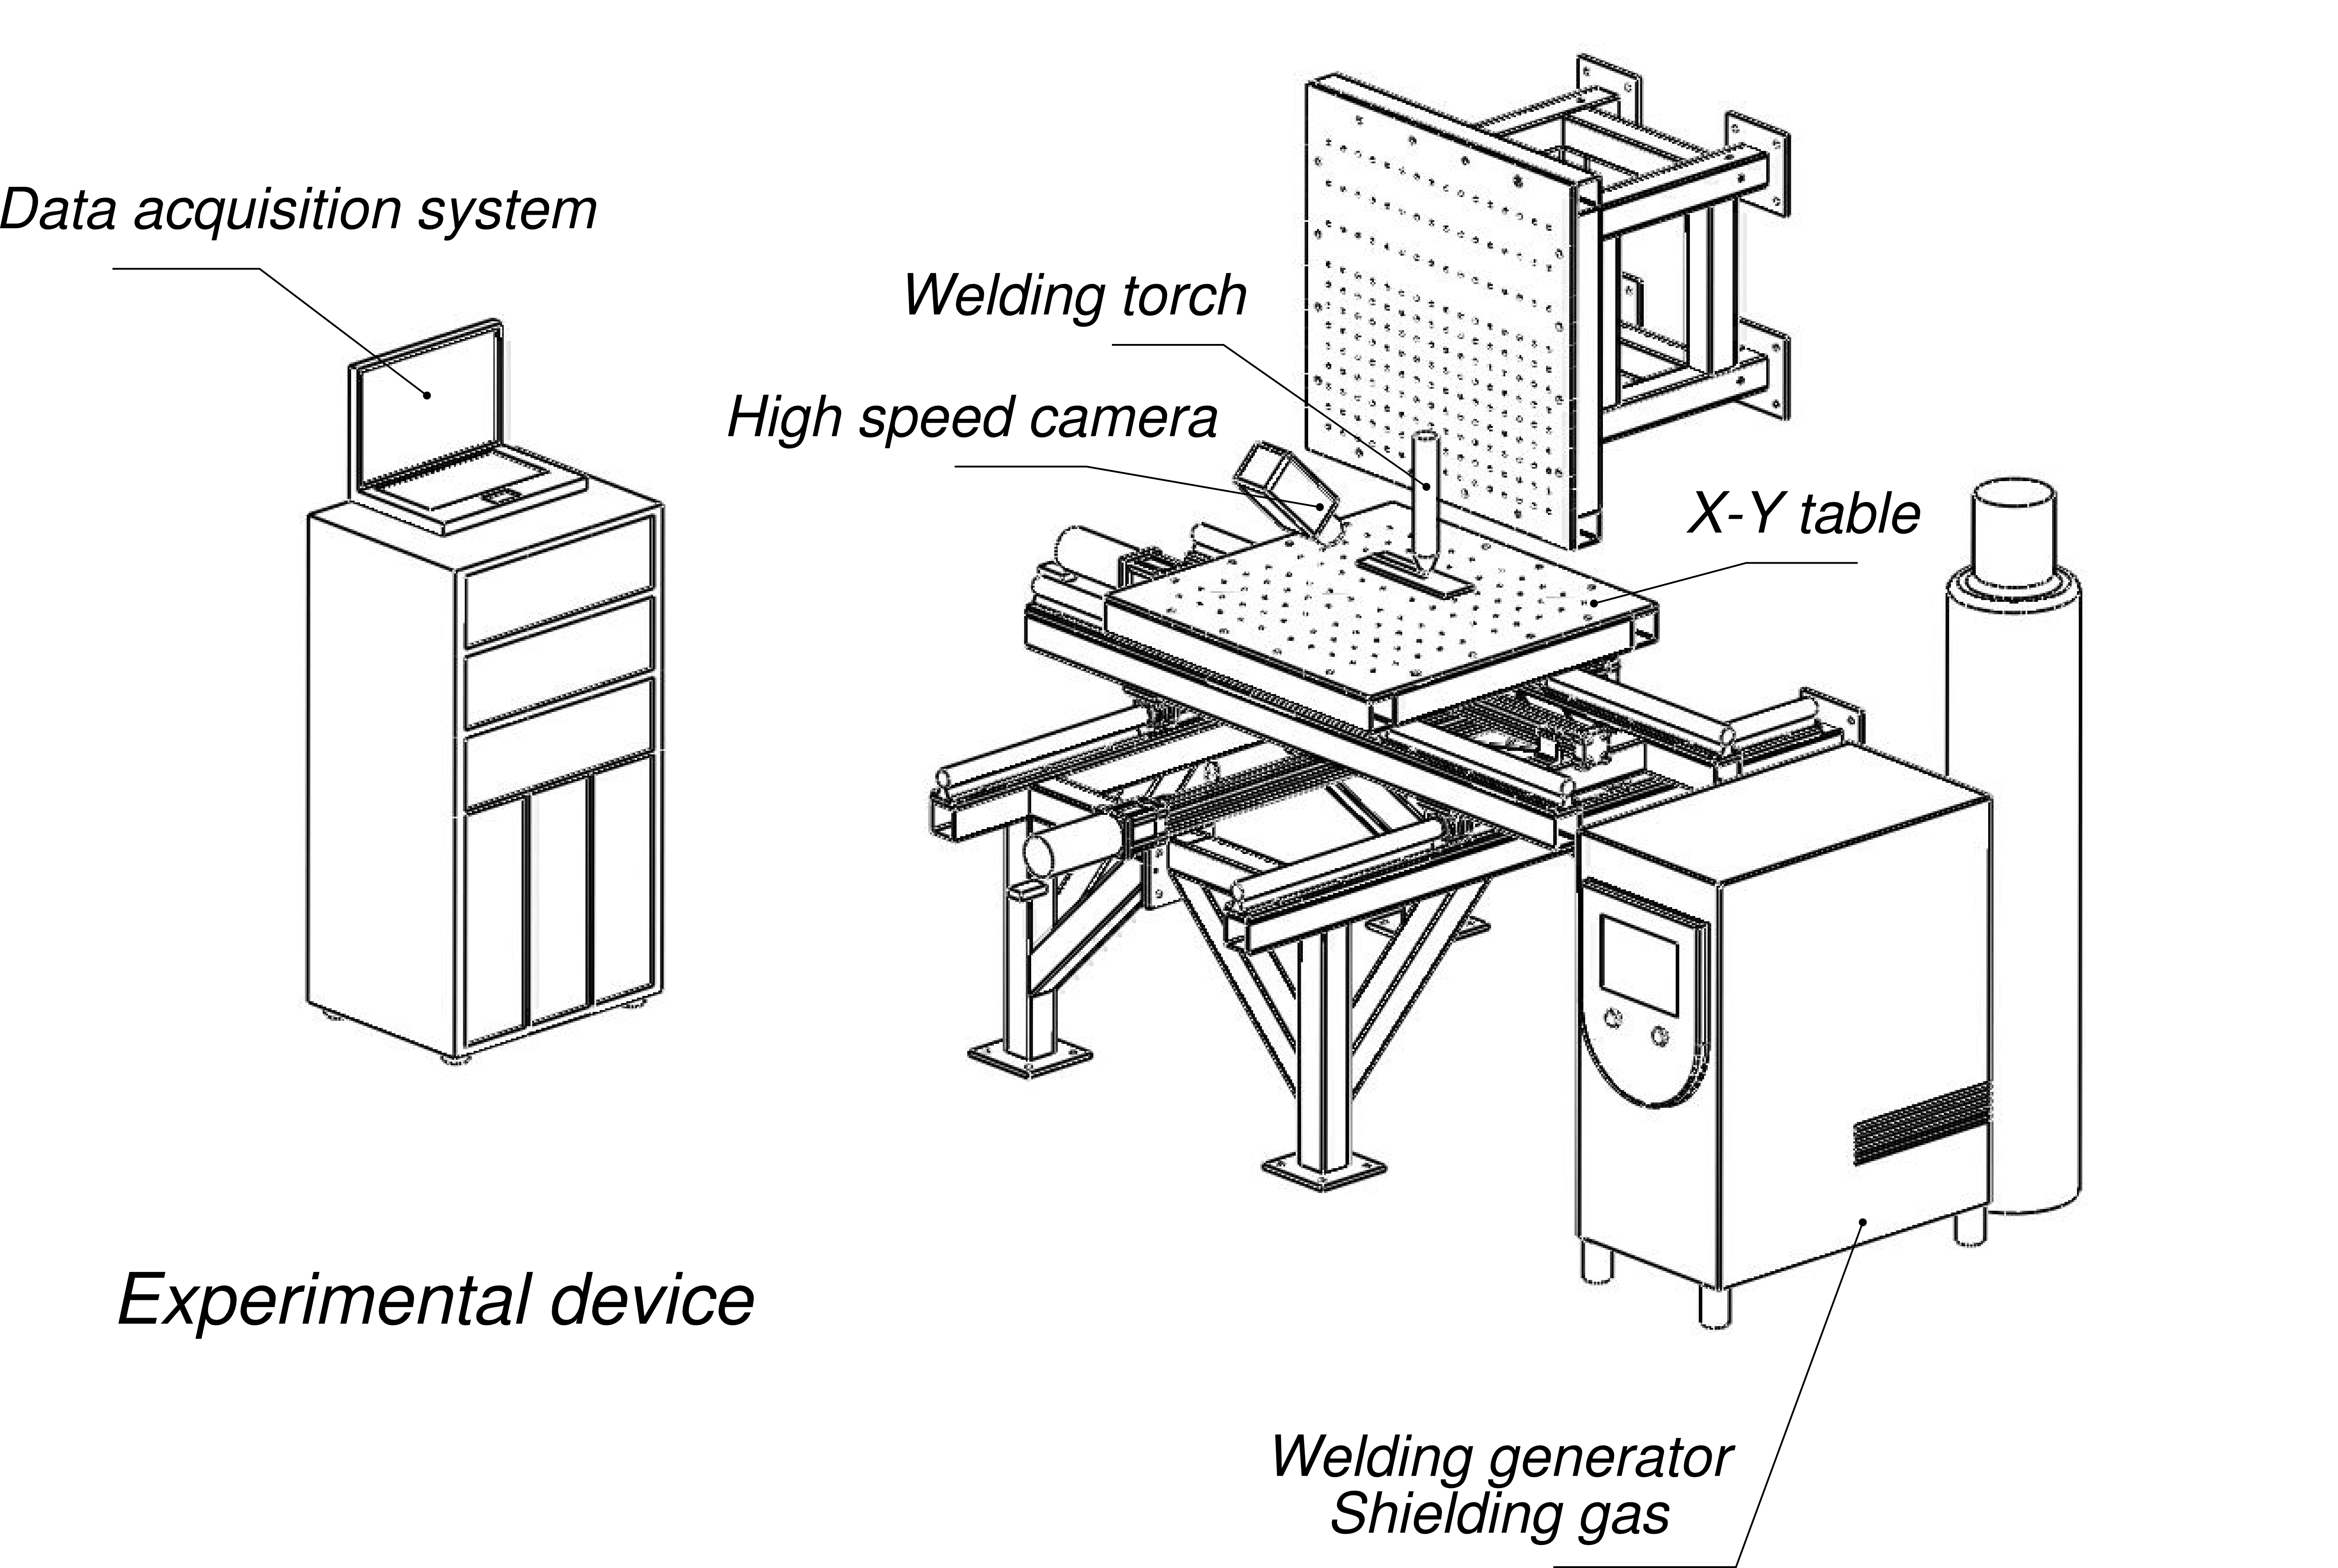
\includegraphics[width=7cm,height=4cm]{schema-platform.png}
%\caption{{\small Experimental platform and specific device}}
%\label{schema-platform}
%\end{center}
%\end{figure}

To compare and analyze the data two open source numerical libraries have been developed: The BAME (multi-physics measures data base) for all general data and the erCv specific to image treatment (including the spreading of welding pool geometry during welding).




\subsection{ Image acquisition setup}
\label{image_acquisition_setup}

Using a similar technique employed by Kovacevic et al. \cite{KOVACEVIC}, the GTAW static process has been recorded by the specular reflection optical method. A $650\ nm$ laser diode has been used to light the weld process from an estimate angle of $35\ degree$. The laser beam width ($ $) has been enough to guarantee a homogeneous illumination of the welding process. The laser projected an image of welding objects (weld pool and surrounding metal substrate) by reflection to the other side of the welding place. At this place and aligned with the optical path of reflected laser beam, a Phantom V5.0 high speed camera has been placed in order to record the images of the process (see figure \ref{schema-montage-experimental-GTAW}). 

%\begin{figure}
%\begin{center}
%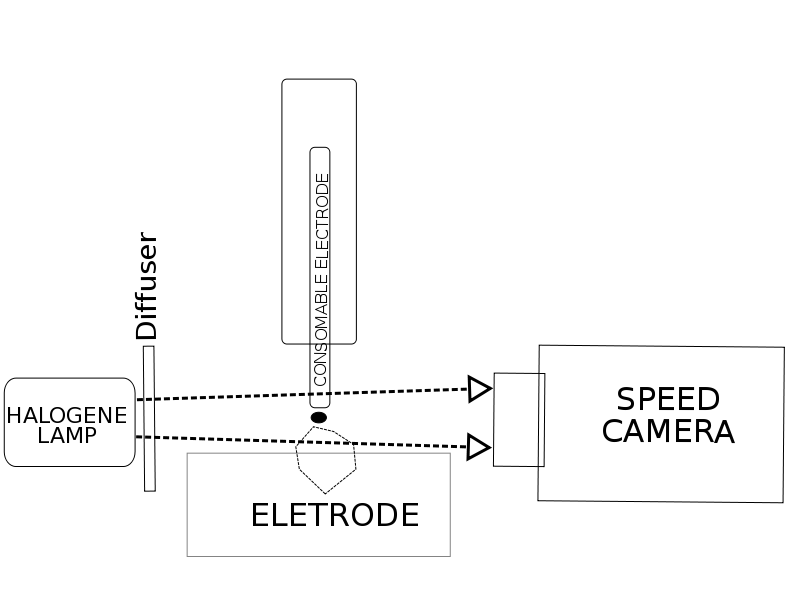
\includegraphics[width=7cm,height=4cm]{schema-montage-experimental-GMAW.png}
%\caption{{\small Experimental setup to detect weld pool edges in GTAW process}}
%\label{schema-montage-experimental-GTAW}
%\end{center}
%\end{figure}

To enhance the image contrast of the weld objects inside the electric discharge, the intensity rate between arc light and laser diode have to be reduce. In order to this a $650\ \pm 10\ nm$ band pass filter, which correspond to the laser diode wavelength, has been placed in front of the camera lens to attenuate the arc light. Nevertheless, the raw images remain highly noisy due to the arc light intensity and disturbed by the non-homogeneous reflections over the dynamic and non-flat weld pool surface. 


% ON CONTINUE ICI
\subsection{ Welding condition}
\label{ welding_conditions}


      
      
\subsection{Weld pool geometrical parameters}
\label{weld-pool-geometrical-parameters}


The purpose is to study the evolution of weld pool object surface and shape in a GTAW process. Therefore it is necessary to detect the contour of the weld pool and calculate the surface area enclose by this. 

%\begin{figure}
%\begin{center}
%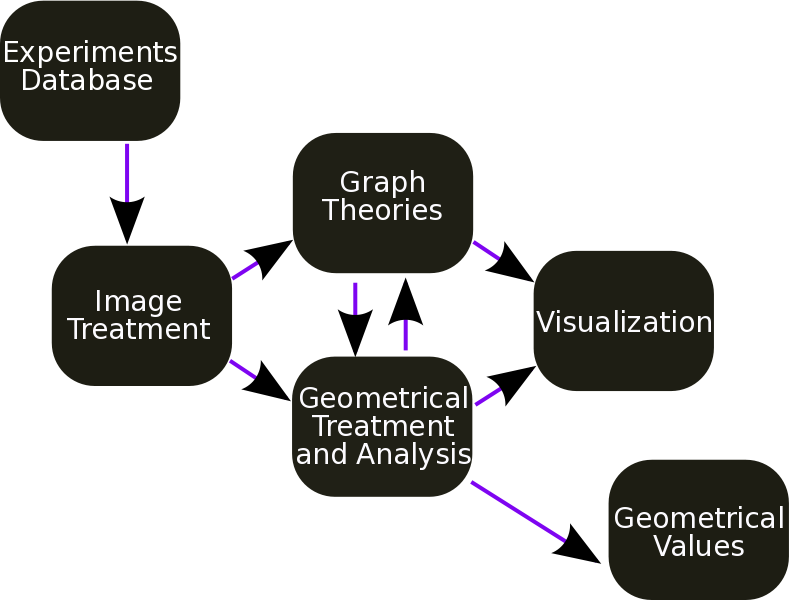
\includegraphics[width=7cm,height=4cm]{schema-erCv.png}
%\caption{{\small Overview schematics of welding objects in a GTAW process}
%\label{schema-macro-drop-droplet-parameters}
%\end{center}
%\end{figure}

At figure \ref{figure_1} appears the geometrical elements to be study at the weld pool: the weld pool contour and surface area.



\section{Image processing tools} 
\label{ image_processing_tools}

Some definitions and brief description of general principles used in
 image processing are required to measure the profiles. Then, the design of the library 
mixing different techniques
is briefly detailed  to detect the profile in the noisy environment.


\subsection{Image treatment basics}
\subsubsection{Some definitions}
\label{some_definitions}

A numerical grey image can be described as 3D surface divided by a grid mesh
 in the X,Y plane. Each square represents a pixel and the relief surface at Z axis,
 the grey level. 
A strong relief change or high gradient greyness values at
 the image are perceived by human eyes as light changes, and can be interpreted
 as objects edges. 

Sometimes, a regular relief patrons or regular greyness
 variation can be distinguished. The human eyes can perceive these patrons as texture 
and interpret the space between different textures zones as edges.
There exist a large spectrum of algorithms to image treatment, in particular for edges detection.
 Most of them can be classified by the way  is operated above the image pixels and grey level.

\subsubsection{Filters}
\label{filters}

The filters are algorithms that operate as mathematical functions $f$ above the 
$X$, $Y$ or both axis of the image ($Z = f(X,Y)$,  
$f(X)$ or $f(Y)$)  modifying his greyness value or $Z$ component. 
Different kind of filters can be mentioned as median, Gaussian, impulse,
 adaptive and others. The impulse filters such Canny are 
widely use to edge detection \cite{COCQUEREZ}. These filters have an
 impulse response to most important greyness gradient in the 
image; this allows the filter a better edges localisation
 (see figure \ref{fig::photo-explication-filter}). 
For this reason, Canny filter is widely 
used in the library to detect the welding elements edges. 
However, it is sensible to noise or secondary greyness gradients in the image
 and, in consequence, it have some difficulties to define closed surface.

\subsubsection{Snake and level set}
\label{snake_and_level_set}
 
Curve propagation is a popular technique in image analysis for object extraction,
 object tracking, edge detection and others (see figure 
\ref{fig::photo-explication-snake}). The central idea behind such an approach
 is to evolve a curve towards the lowest potential of a cost function. 
However at each stage of curve evolution, each curve point potential has
 to be computed. A lot of point (better curve resolution) take a lot 
computing time, and therefore are not yet apply to real time detection
 or relatively speed automatic image processing. For this reason snake algorithms are not used in the library.

\subsubsection{Segmentation}
\label{segmentation}

Let $B$ an image and let $R_{i}$ a region of $B$ such:

\begin{eqnarray}
B = \bigcup_{i}R_{i}\ \forall i \in \{0, \mbox{numbers of regions in B}\} \\
\mbox{with}\ R_{i} \neq \emptyset \\
\mbox{and}\  R_{i}\bigcap R_{j} = \emptyset\ \forall i, j\ \mbox{with}\ i \neq j\ 
\label{equation-segmentation}
\end{eqnarray}

A $B$ segmentation is an image treatment which generate a $B$ partition in $R_{i}$ regions. 
Each region is a connected set of pixels with 
common properties (intensity, texture,...) \cite{COCQUEREZ}.
 The partition is generated by operations or comparisons methods between 
regions. Generally, this treatment offers a good detection edges if
 the elements and surrounding area have different textures (see figure
 \ref{fig::photo-explication-segmentation}). 
Note that different regions can belong to the same partition,
 therefore the surface is not always connected and,
 in consequence, the edges of the interest regions are not always closed.

%\begin{figure}[h!]
%\begin{center}    
%\subfigure[Weld pool image in static GTAW process]{\label{fig::photo-explication-patron}\includegraphics[width=3.5cm,height=3.5cm]{figure3a.png}}
%\subfigure[Canny filter treatment]{\label{fig::photo-explication-filter}\includegraphics[width=3.5cm,height=3.5cm]{figure3b.png}}\\
%\subfigure[Snake treatment]{\label{fig::photo-explication-snake}\includegraphics[width=3.5cm,height=3.5cm]{figure3c.png}}
%\subfigure[Segmentation image by 2 cluster sample comparison]{\label{fig::photo-explication-segmentation}\includegraphics[width=3.5cm,height=3.5cm]{figure3d.png}}
%\end{center}
%\caption{{\small Samples of different methods technique for image processing}}
%\label{fig::photo-explication}
%\end{figure}


\subsection{Image treatment library}
\label{image_treatment_library}

A multipurpose image processing library has been developed 
and currently use at the laboratory, in order to analyze welding process objects.
erCv is able to perform edge detection and geometrical analysis in a different 
welding objects such as Macro drop, droplets and weld pool.
The library can manage different kinds of image acquisition (optical setup). 
The library is implemented in a oriented object C++ language.
Then,  erCv is a scalable 
and portable library able to perform real time
 contour detection. The library is implemented in  C++ with some bindings in python,
 making it relatively convivial to use for non-programmers.
To manage the edge detection during welding process,
the library is composed by four processing modules: 
\begin{description}
\item[Image Treatment:] Due to weld process conditions such arc lightening, 
 heat and electrodes positions; the raw image registered by CCD 
 camera are not calibrated and present light inhomogeneities and 
 noise. In order to obtain the real shape and size of weld elements, this module 
 includes calibration algorithms. To detect the welding objects contours it is 
 necessary to improve the weld element image. This module has the 
 pre-processing treatments for noise reduction and image enhancement.
 Then to start the edges detection process, this module includes processing
 algorithms as segmentation by samples comparator, watershed transformation,
 filters edge detectors and histogram based methods.  
 Most of the functionality comes from \cite{OPENCV}.
\item[Geometrical Treatment and Analysis:] This module convert edges pixels points into connected 
   segments to conclude the edge detection
  process, completing and in some cases extrapolating the weld
  elements edge. It is also responsible to compute the geometrical 
  data of welding elements such weld pool surface and metal transfer drop volumes. 
  This module uses a full geometry algorithm library\cite{CGAL}, which include different algorithms
  such as triangulations and mesh generation, alpha shape and 
  convex hull generation and polygonal structures.
\item[Graph Theories:] To compute the geometrical data of welding elements
   it is necessary to extract the welding object edge from the image; this
   required some criteria such as continuity, length or closing condition.
   This module use graph algorithms to  identify and select the welding element edge using the
   criteria. This module is composed by connected segments, estimates
   minimal cut, determine largest chain segments and others algorithms. 
   The algorithm of \cite{BOOSTGRAPH} are used.
\item[Visualization:] This module is a set of 
  functions use to execute, show and/or register the 
  different steps at the image process.
\end{description}

%\begin{figure}
%\begin{center}
%\includegraphics[width=10cm]{figure4.png}
%\caption{{\small Flow diagram of erCv library composition}}
%\label{fig::schema-erCv}
%\end{center}
%\end{figure}

The originality of the library comes from the aggregation 
and complementarity of the different numerical tools.
The main difficulty is to find algorithms with good parameters all along the process.

% On s ARRETE LA

\section{ Applying image processing}
\label{ applying_image_processing}

\subsection{ Image Features}
\label{image_features}

Before to propose an effective procedure using filtering or segmentation algorithms from erCv library, some image features imposed by the image acquisition procedure as: image view angle and image color, must be analyzed and modified. 


\subsubsection{ Image Calibration}
\label{ image_calibration}

As was shown in section \ref{image-acquisition-setup}, the camera records a specular reflection of the welding process. Therefore the image of the welding objects is not orthogonal to the optical axes of the camera. In order to correct the image perspective, a function has been included in the image treatment module. A control image (small chessboard image with known real dimensions) is recorded at the weld pool place. An algorithm recognizes the chessboard corners and builds a transformation matrix between the control image (chessboard recorded image) and the original digital image. Finally, to calibrate the image dimension (in pixels) to the real objects dimension (in millimeters), a conversion scale is applied with the real dimensions of chessboard control image $conv = 1\ mm/ 20\ pixels$. 

%\begin{figure}[h!]
%\begin{center}    
%\subfigure[Chessboard control image]{\label{photo-calibration-cuadro-patron}\includegraphics[width=3.5cm,height=3.5cm]{photo-calibration-cuadro-patron.png}}
%\subfigure[Chessboard original digital image]{\label{photo-calibration-cuadro-origin}\includegraphics[width=3.5cm,height=3.5cm]{photo-calibration-cuadro-origin.png}}\\
%\subfigure[Raw recorded image]{\label{photo-calibration-image-origin}\includegraphics[width=3.5cm,height=3.5cm]{photo-calibration-image-origin.png}}
%\subfigure[Perspective corrected image]{\label{photo-calibration-image-corrected}\includegraphics[width=3.5cm,height=3.5cm]{photo-calibration-image-corrected.png}}
%\end{center}
%\caption{{\small Perspective image correction samples}}
%\label{photo-calibration}
%\end{figure}



\subsubsection{Image color}
\label{image-color}

As has been mentioned in section \ref{filters}, most of the filter type algorithm (including canny filter) operates as function over the image grayness levels. Moreover, the segmentation processing requires less computing time over 1-channels image than over 3-channels image. In order to allow to use filters algorithm and to do more efficient the image processing a function has been include into the treatment module to convert the color weld pool image to gray level image (see image \ref{photo-weldpool-grayness}).


  
  \subsection{ Image Preprocessing}
\label{image-preprocessing}


The idea is to recognize the weld pool from the raw image and therefore calculate his 2D surface area. This requires the identification of a well define weld pool contour. Several approaches could be uses to obtain the weld pool contour such as edge detection techniques  ( impulse filters) \cite{WU2}, Hough transforms \cite{OLSON} or geometrical weld pool division \cite{KOVACEVIC}. Nevertheless the most common approach is the image segmentation \cite{WANG}. 

Thanks to the optical method acquisition (specular reflection), the mirror like surface of the weld pool reflect a uniform dark surface to the camera while the solid metal surface reflect a diffuse lighting surface \cite{WU2}.

A natural way to segment the images, could be separate it between the roughness (non homogeneous lighting zone) and non roughness zone or dark zone as the weld pool area (see figures \ref{photo-macro-drop-original}). 

However the low intensity contrast between the weld pool and the surrounding solid metal due to the radiation from the pool, as well as the impurities or oxides presents on the weld pool (see figure \ref{photo-macro-drop-original}), prevents to use a simply approach of existing techniques to isolate the weld pool. Perform 2D contour require an effective techniques combination, to correct the light reflection distortion into the weld pool, isolate the weld pool and extract his contour.
% ; using to this the basic image processing concepts previous mentioned (see section
% \ref{image-processing-background}). 



\subsubsection{Impurities and reflex correction}
\label{impurities-and-reflex-correction}

To apply segmentation techniques able to isolate the weld pool from the image, the arc reflects and the impurities over the weld pool have to be reduced. 

Note that the impurities and the high intensities reflection appear as white or high gray level blobs into the dark or homogeneous low gray level weld pool (see figure \ref{photo-grayness-level}. An algorithm able to detect the ��white�� blobs into the weld pool and correct its has been developed and included into the image treatment module of erCv. The algorithm use the same principia used by the well known red eye detections and corrections algorithm \cite{GAUBATZ}.

The white blob correction algorithm uses three threshold values to fix the blob selection criteria: $g\_upper$ to define the minimal gray level of the ��white blob��, $g\_lower$ to define the maximal gray level of the weld pool and $s\_max$ to define the blob maximum pixel sizes. 

Call $B$ an arbitrary ��white�� blob set, $\partial B$ his boundary and $size(B)$ his size in pixels numbers. Call $(x, y)$ a pixel coordinates in the image and $gray\_level( x, y)$ the pixel associate grayness level.

 \begin{eqnarray*}
 ( x, y) \in B\ \mbox{if} \\
gray\_level( x, y) > g\_upper \\
\mbox{Then}\ B\ \mbox{is in the weld pool if} \\
gray\_level( x, y)\ \leq\ g\_lower\ \forall\ (x,y)\  \in\  \partial B \\ 
\mbox{and if}\ size(B)\ <\ s\_max
 \end{eqnarray*}
 
If $B$ is in the weld pool, the grayness level at each pixel $(x,y)$ inside $B$ is replaced by the grayness average value of the grayness level pixels of $\partial B$ (see equation \ref{equation-grayness-recouvrement}). Then the ��white�� blob is replaced by a low average grayness level surface, similar to the rest of the weld pool grayness level. 

\begin{equation}
gray\_level( x, y) = \frac{gray\_level( x, y_{\partial B}) + gray\_level( x_{\partial B}, y) }{ 2}
\label{equation-grayness-recouvrement}
\end{equation}

Using this algorithm, most of the impurities and the arc light reflections into the weld pool have been corrected.
	


\subsubsection{ Texture Analysis Principia}
\label{texture-analysis-principia}

Now, the weld pool appears as a more uniform dark surface, which contrast with the non uniform gray level values of the surrounding solid metal area.
This particularity in the grayness level distribution (roughness) at the image could be interpreted as different textures zones \cite{MATERKA}, in the same the way as the eyes recognize the texture in the object surface and$/$or images. 

The texture analysis method to perform image segmentation is an image processing technique widely uses in biomedicine, satellite recognition, industrial quality control and others fields requiring image processing. There exist different approaches to texture analysis, each one using their own image analysis methods: Structural, statistical, model based and transform methods \cite{MATERKA}.
The structural method requires complex logical analysis, while the transform and model based methods require mathematical analysis that required deterministic properties in grayness levels distributions \cite{MATERKA}. The statistical methods respond intuitively to what human eyes recognize: Two surfaces with different grayness level distribution or roughness.

As has been mentioned in section \ref{segmentation}, image segmentation means split into two or more fields the image. One field, would be mark in one color and the rest of the image in other color \cite{COCQUEREZ}.

\subsubsection{ Applying texture analysis}
\label{appliying-texture-analysis}



              
%\begin{figure}[h!]
%\begin{center}    
%\subfigure[Macro drop raw image]{\label{fig::photo-macro-drop-patron}\includegraphics[width=3.5cm,height=3.5cm]{figure5a.png}}
%\subfigure[Macro drop grayness image]{\label{fig::photo-macro-drop-grey}\includegraphics[width=3.5cm,height=3.5cm]{figure5b.png}}\\
%\subfigure[First smooth filter]{\label{fig::photo-macro-drop-smoothblur}\includegraphics[width=3.5cm,height=3.5cm]{figure5c.png}}
%\subfigure[Adaptive threshold per regions]{\label{fig::photo-macro-drop-adaptivethreshold}\includegraphics[width=3.5cm,height=3.5cm]{figure5d.png}}\\
%\subfigure[Median filter]{\label{fig::photo-macro-drop-smoothmedian}\includegraphics[width=3.5cm,height=3.5cm]{figure5e.png}}
%\subfigure[Canny filter]{\label{fig::photo-macro-drop-canny}\includegraphics[width=3.5cm,height=3.5cm]{figure5f.png}}\\
%\end{center}
%\caption{{\small Image treatment step by step of PGMAW process}}
%\label{fig::photo-macro-drop}
%\end{figure}


\subsection{Edge extraction}
\label{edge_extraction}


 
%\begin{figure}[h!]
%\begin{center}    
%\subfigure[t1 ]{\label{fig::photo-results-macro-drop-t1}\includegraphics[width=3.5cm,height=3.5cm]{figure6a.png}}
%\subfigure[t2 ]{\label{fig::photo-results-macro-drop-t2}\includegraphics[width=3.5cm,height=3.5cm]{figure6b.png}}\\
%\subfigure[t3 ]{\label{fig::photo-results-macro-drop-t3}\includegraphics[width=3.5cm,height=3.5cm]{figure6c.png}}
%\subfigure[t4 ]{\label{fig::photo-results-macro-drop-t4}\includegraphics[width=3.5cm,height=3.5cm]{figure6d.png}}\\
%\end{center}
%\caption{{\small Images series of macro drop profiles}}
%\label{fig::photo-results-macro-drop}
%\end{figure}
%
%               
%                                  
%\begin{figure}[h!]
%\begin{center}    
%\subfigure[t = ]{\label{fig::photo-droplet-canny}\includegraphics[width=3.5cm,height=3.5cm]{figure7a.png}}
%\subfigure[t = ]{\label{fig::photo-droplet-alpha-shape}\includegraphics[width=3.5cm,height=3.5cm]{figure7b.png}}\\
%\end{center}
%\caption{{\small Images series of macro drop profiles}}
%\label{fig::photo-results-droplet}
%\end{figure}

A graph algorithm connects this segment and finds the longest closer segment.
 The longest closer segment corresponds to the metal transfer drop profile 
(see figure \ref{fig::photo-results-droplet}).

%\begin{figure}[h!]
%\begin{center}    
%\subfigure[t1 ]{\label{fig::photo-results-droplet-t1}\includegraphics[width=3.5cm,height=3.5cm]{figure8a.png}}
%\subfigure[t2 ]{\label{fig::photo-results-droplet-t2}\includegraphics[width=3.5cm,height=3.5cm]{figure8b.png}}\\
%\subfigure[t3 ]{\label{fig::photo-results-droplet-t3}\includegraphics[width=3.5cm,height=3.5cm]{figure8c.png}}
%\subfigure[t4 ]{\label{fig::photo-results-droplet-t4}\includegraphics[width=3.5cm,height=3.5cm]{figure8d.png}}\\
%\end{center}
%\caption{{\small Images series of macro drop profiles}}
%\label{fig::photo-results-droplet}
%\end{figure}



\subsection{Geometrical Analysis}
\label{geometrical_analize}


\section{ Results}
\label{results}


\subsubsection{Discussions}
\label{discussion}




\section{ Conclusions}
\label{conclusions}



\section*{Acknowledgment}
The authors want to thanks the Agence National pour la Recherche (ANR) which grants this research
under the ANR-JCJC038 young scientist contract. 
\section*{References}
$ $
%\bibliographystyle{unsrt}
\bibliography{paper_bain_drop}

%\section*{References}
%\begin{thebibliography}{10}
%\bibitem{book1} Goosens M, Rahtz S and Mittelbach F 1997 {\it The \LaTeX\ Graphics Companion\/} 
%(Reading, MA: Addison-Wesley)
%\bibitem{eps} Reckdahl K 1997 {\it Using Imported Graphics in \LaTeX\ } (search CTAN for the file `epslatex.pdf')

% \cite{BALSAMO}
%\cite{WANG}
%\cite{CHO}
%\cite{LIN}
% \cite{ZHANG4}
%\cite{BAE}
%\cite{NORDBRUCH}
%\bibitem{CGAL} http://www.cgal.org 
%\cite{ChapuisThesis}
%\cite{WU1}
%\cite{SEED}
% \cite{COCQUEREZ}
% \cite{OPENCV}
% \cite{GEOMETRICAL}
% \cite{white}
%\end{thebibliography}
\end{document}

